% ---------
%  Compile with "pdflatex hw1".
% --------
%!TEX TS-program = pdflatex
%!TEX encoding = UTF-8 Unicode

% Template borrowed from Jeff Erickson.

\documentclass[11pt]{article}
\usepackage[utf8]{inputenc}		% Allow some non-ASCII Unicode in source
\usepackage{jeffe, handout,graphicx}
\usepackage{forest}
\usepackage{mathtools}
\usepackage{tikz, ifthen, etoolbox}
\usepackage{float}
\usetikzlibrary{positioning}
\newcommand{\pd}{\partial}
\newcommand{\bs}{\boldsymbol}
\newcommand{\ifstringequal}[4]{%
  \ifnum\pdfstrcmp{#1}{#2}=0
  #3%
  \else
  #4%
  \fi
}


% =========================================================
%   Define common stuff for solution headers
% =========================================================
\Class{CS 6301.503}
\Semester{Spring 2019}
\Authors{1}
\AuthorOne{Scott C. Waggener}{scw180000}
%\Section{}

% =========================================================
\begin{document}
\HomeworkHeader{3 (Calculus)}{1}% homework number, problem number
% ---------------------------------------------------------
\noindent
\begin{solution}
	Complete
\end{solution}

% =========================================================
\HomeworkHeader{3 (Calculus)}{2}% homework number, problem number
% ---------------------------------------------------------
\begin{solution}
	Complete
\end{solution}

% =========================================================
\HomeworkHeader{3 (Calculus)}{3}% homework number, problem number
% ---------------------------------------------------------
\begin{solution}
	Complete
\end{solution}

% =========================================================
\HomeworkHeader{3 (Calculus)}{4}% homework number, problem number
% ---------------------------------------------------------
Let $\boldsymbol{x}$ be the $K \times 1$ vector output of the last layer of a
xNN and
$e = \text{crossEntropy}(\boldsymbol{p}^*,\text{softMax}(\boldsymbol{x}))$
be the error where $\boldsymbol{p}^*$ is a $K \times 1$ vector with a $1$ in
position $k^*$ representing the correct class and $0$s elsewhere. Derive
$\pd e/ \pd\boldsymbol{x}$

\begin{solution}
	\begin{align}
		\frac{\pd e}{\pd \bs{x}} &=
		\begin{pmatrix}
			p(x_{0}) \\
			\vdots \\
			p(x_{k})-1 \\
			\vdots \\
			p(x_{n})
		\end{pmatrix}
		\begin{matrix}
			\phantom{p(x_{0})} \\
			\phantom{\vdots} \\
			\leftarrow k \phantom{p(x_{k})-1} \\
			\phantom{\vdots} \\
			\phantom{p(x_{n})} \\
		\end{matrix}
	\end{align}
\end{solution}

\begin{proof}
	First, note that error function $e$ is given by the cross entropy of a
	softmax, the typical error function chosen for \textbf{classification}
	networks. We can tell by the given error function that we will need to
	apply the chain rule.
	Specifically, we will need to compute the following for use in the chain
	rule.

	\begin{align}
		\frac{d}{d \bs{x}} \text{softMax}(\bs{x})
		&&
		\frac{\pd}{\pd \bs{p}} \text{crossEntropy}(\bs{p}^*, \bs{p})
	\end{align}

	We will start with cross entropy. Recall that cross entropy is given by

	\begin{align}
		\text{crossEntropy}(\boldsymbol{p}^*, \boldsymbol{p})
		\equiv
		c(\boldsymbol{p}^*, \boldsymbol{p})
		=
		-\sum_{x_i\in\boldsymbol{x}} p^*(x_i) \log p(x_i)
	\end{align}

	Differentiating cross entropy for each of $x_i \in \bs{x}$ produces a
	gradient vector. We know that $\bs{p}^*$ is a one hot vector at position
	$k$ meaning that our gradient will be nonzero only at position $k$ upon
	differentiation. Applying the log derivative identity gives

	\begin{align}
		\nabla_{\bs{x}}\bigg(-\sum_{x_i\in\bs{x}} p^*(x_i) \log p(x_i)\bigg)
 		&=
		\begin{pmatrix}
			-\frac{\pd}{\pd x_1} p^*(x_1) \log p(x_1)\\
			-\frac{\pd}{\pd x_2} p^*(x_2) \log p(x_2)\\
			\vdots \\
			-\frac{\pd}{\pd x_k} p^*(x_k) \log p(x_k)\\
			\vdots \\
			-\frac{\pd}{\pd x_N} p^*(x_N) \log p(x_N)
		\end{pmatrix}
		&=
		\begin{pmatrix}
			0 \\
			0 \\
			\vdots \\
			\underbrace{-\frac{\pd}{\pd x} \log p(x_k)}_{-1 / p(x_k)} \\
			\vdots \\
			0
		\end{pmatrix}
		\\ &=
		\begin{pmatrix}
			0 \\
			0 \\
			\vdots \\
			-\frac{1}{p(x_k)} \\
			\vdots \\
			0
		\end{pmatrix}
		\begin{matrix}
			\phantom{0} \\
			\phantom{0} \\
			\phantom{\vdots} \\
			\leftarrow k \phantom{\frac{1}{1}} \\
			\phantom{\vdots} \\
			\phantom{0}
		\end{matrix}
	\end{align}

	So our cross entropy gradient for a one hot vector $\bs{p}^*$ with nonzero
	position $k$ is $0$ everywhere except at position $k$.
	\newline

	Now we compute our next required derivative: softmax.
	The softmax function is given by

	\begin{align}
		\text{softMax}(\boldsymbol{x})
		&=
		\frac{1}{
			\Sum_{x_i\in\bs{x}}e^{x_i}
		}
		\begin{pmatrix}
			e^{x_0} \\
			e^{x_1} \\
			\vdots \\
			e^{x_K}
		\end{pmatrix}
	\end{align}

	Calculating this derivative will yield a Jacobian matrix

	\begin{align}
		\frac{\pd s}{\pd \bs{x}}
		&=
		\Bigg(\Sum_{x_i\in\bs{x}}e^{x_i}\Bigg)^{-1}
		\frac{\pd}{\pd\bs{x}}
		\begin{pmatrix}
			e^{x_0} \\
			e^{x_1} \\
			\vdots \\
			e^{x_K}
		\end{pmatrix}
		+
		\frac{\pd}{\pd \bs{x}} \Bigg(\Sum_{x_i\in\bs{x}}e^{x_i}\Bigg)^{-1}
		\begin{pmatrix}
			e^{x_0} \\
			e^{x_1} \\
			\vdots \\
			e^{x_K}
		\end{pmatrix}
		\\
		&=
		\underbrace{
			\Bigg(\Sum_{x_i\in\bs{x}}e^{x_i}\Bigg)^{-1}
			\begin{pmatrix}
				e^{x_0} & 0 & \cdots & 0 \\
				0 & e^{x_1} & \cdots & 0 \\
				\vdots & \vdots & \ddots & \vdots \\
				0 & 0 & \cdots & e^{x_n} \\
			\end{pmatrix}
		}_{
			\begin{aligned}
				&s(\bs{x})\vert i &\forall i=j \\
				&0 &\forall i\neq j \\
			\end{aligned}
		}
		-
		\underbrace{
			\Bigg(\Sum_{x_i\in\bs{x}}e^{x_i}\Bigg)^{-2}
			\begin{pmatrix}
				e^{2 x_0} & e^{x_1 + x_0}  & \cdots & e^{x_n + x_0} \\
				e^{x_0 +x_1} & e^{2 x_1} & \cdots & e^{x_n + x_1} \\
				\vdots & \vdots & \ddots & \vdots \\
				e^{x_0 + x_n} & e^{x_1 + x_n}  & \cdots & e^{2 x_n} \\
			\end{pmatrix}
		}_{
			\begin{aligned}
				&s(\bs{x})^2\vert i &\forall i=j \\
				&s(\bs{x})\vert i\cdot
					s(\bs{x})\vert j
					&\forall i\neq j \\
			\end{aligned}
		}
		\\
	\end{align}

	In this Jacobian matrix the entries come from two possible
	cases that can both be expressed in terms of the original function. To express
	this more cleanly let us denote the softmax at a given $x_i \in \bs{x}$
	with the same $p(x_i)$ notation used for handling cross entropy.
	Then the entry of the $i$th row and $j$th column in the Jacobian matrix for
	softmax of vector $\bs{x}$ will be given by

	\begin{align}
		J_s(\bs{x})_{i j} &= \begin{cases}
			p(x_i) - p(x_i)^2 & \forall i=j \\
			- p(x_i) \cdot p(x_j) & \forall i\neq j
		\end{cases}
	\end{align}

	Now we have found what we need to apply the chain rule

	\begin{align}
		\frac{\pd e}{\pd \bs{x}} &= \bs{J}_s(\bs{x})
		\cdot
		\nabla_{\bs{x}}c(\bs{p}^*, \bs{p})
		\\
		&=
		\begin{pmatrix}
			p(x_{0}) - p(x_{0})^2
				& - p(x_{0})\cdot p(x_{1})
				& \cdots
				& -p(x_{0})\cdot p(x_{n})
			\\
			-p(x_{1}) \cdot p(x_{0})
				& p(x_{1})-p(x_{1})^2
				& \cdots
				& -p(x_{1})\cdot p(x_{n})
			\\
			\vdots
				& \vdots
				& \ddots
				& \vdots
			\\
			-p(x_{n}) \cdot p(x_{0})
				& -p(x_{n})\cdot p(x_{1})
				& \cdots
				& p(x_{n}) - p(x_{n})^2
		\end{pmatrix}
		\cdot
		\begin{pmatrix}
			0 \\
			\vdots \\
			-\frac{1}{p(x_k)} \\
			\vdots \\
			0
		\end{pmatrix}
		\\
		&=
		\begin{pmatrix}
			\frac{p(x_{0}) \cdot p(x_{k})}{p(x_k)} \\
			\vdots \\
			\frac{p(x_{k})^2 - p(x_{k})}{p(x_k)} \\
			\vdots \\
			\frac{p(x_{n}) \cdot p(x_{k})}{p(x_k)} \\
		\end{pmatrix}
		\\
		\frac{\pd e}{\pd \bs{x}}
		&=
		\begin{pmatrix}
			p(x_{0}) \\
			\vdots \\
			p(x_{k})-1 \\
			\vdots \\
			p(x_{n})
		\end{pmatrix}
		\begin{matrix}
			\phantom{p(x_{0})} \\
			\phantom{\vdots} \\
			\leftarrow k \phantom{p(x_{k})-1} \\
			\phantom{\vdots} \\
			\phantom{p(x_{n})} \\
		\end{matrix}
	\end{align}

	This result is very clean and intuitive. It shows that increasing the
	probabilities for incorrect labels increases error, and that decreasing
	probability for the correct label increases error. We were able to get this
	result by treating softmax and cross entropy derivatives together via the
	chain rule. This property can only be exploited in implementation by using
	procedures in the library that treat these layers together.

\end{proof}

% ---------------------------------------------------------
\HomeworkHeader{3 (Calculus)}{5}% homework number, problem number
% ---------------------------------------------------------

\begin{solution}
	\begin{align}
		\frac{\pd e}{\pd \bs{x}}
		&=\bigg(\bs{H}^T \cdot \bs{I}_n\cdot\bs{I}_n\{0, 1\}\cdot
			\bs{I}_n\cdot\frac{\pd e}{\pd \bs{y}}\bigg)
		+
		\bs{I}_n
	\end{align}
\end{solution}

\begin{proof}
	First we decompose the residual block representing the flow of information
	in backpropagation: residual input, pointwise nonlinearity, bias vector,
	and dense layer.

	\tikzset{%
		every block/.style={
			rectangle,
			draw,
			minimum width=2cm,
			minimum height=1cm,
			node distance=4cm
		},
		block backward/.style={
			rectangle,
			draw,
			minimum width=2cm,
			minimum height=1cm,
			node distance=4cm,
			color=red
			%execute at begin node=\color{black}$\vdots$
		},
		phantom node/.style={
			rectangle,
			draw=none,
			minimum width=1cm,
			minimum height=1cm,
			node distance=2cm
		}
	}

	\begin{figure}[H]
	\centering
	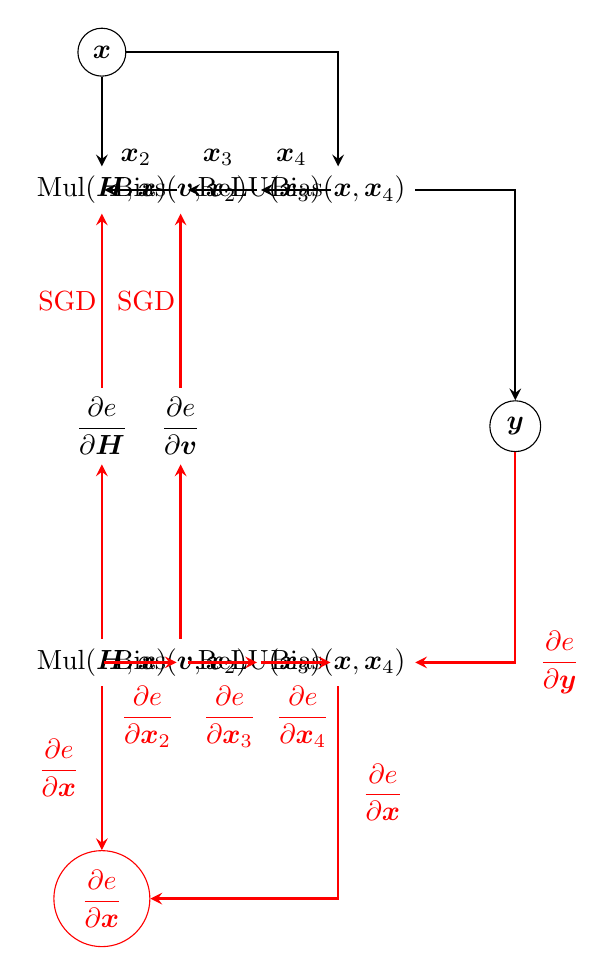
\begin{tikzpicture}[x=1.5cm, y=1.5cm, >=stealth]

		% Dense
		\node [every block/.try, block forw-1/.try] (forw-1) at (0,4) {
			Mul$(\bs{H}, \bs{x})$
		};
		\node [block backward/.try, block forw-1/.try] (back-1) at (0,0) {
			Mul$(\bs{H}, \bs{x})$
		};
		\node [block backward/.try, block forw-1/.try] (h-1) at (0,2) {
			$\dfrac{\pd e}{\pd \bs{H}}$
		};

		% Bias
		\node [every block/.try, block forw-2/.try, right of=forw-1] (forw-2) {
			Bias$(\bs{v}, \bs{x}_2)$
		};
		\node [block backward/.try, block back-2/.try, right of=back-1] (back-2) {
			Bias$(\bs{v}, \bs{x}_2)$
		};
		\node [block backward/.try, block forw-2/.try, right of=h-1] (h-2) {
			$\dfrac{\pd e}{\pd \bs{v}}$
		};

		% RELU
		\node [every block/.try, block forw-3/.try, right of=forw-2] (forw-3)  {
			ReLU$(\bs{x}_3)$
		};
		\node [block backward/.try, block back-3/.try, right of=back-2] (back-3)  {
			ReLU$(\bs{x}_3)$
		};
		\node [block backward/.try, block forw-2/.try, right of=h-2, draw=none] (h-3) { };

		% Residual bias
		\node [every block/.try, block forw-4/.try, right of=forw-3] (forw-4)  {
			Bias$(\bs{x}, \bs{x}_4)$
		};
		\node [block backward/.try, block back-4/.try, right of=back-3] (back-4)  {
			Bias$(\bs{x}, \bs{x}_4)$
		};
		\node [block backward/.try, block forw-2/.try, right of=h-3, draw=none] (h-4) {
		};

		% x input
		\node [circle, draw, above of=forw-1, node distance=1.75cm] (xin) {$\bs{x}$};

		% y output
		\node [circle, draw, right of=h-4, node distance=2.25cm]
			(y) {$\bs{y}$};

		\draw [->, line width=0.3mm] (forw-4) -| (y);
		\draw [->, line width=0.3mm] (xin) -- (forw-1);
		\draw [->, line width=0.3mm] (xin) -| (forw-4);
		\draw [->, line width=0.3mm, color=red] (y) |-
			node [text width=0.5cm,midway, right=0.5em] {
				$\dfrac{\pd e}{\pd \bs{y}}$
			}
			(back-4);

		\foreach \l [count=\i] in {2, 3, 4}
			\draw [->, line width=0.3mm] (forw-\i) --
				node [text width=0.5cm,midway,above=0.5em] {$\bs{x}_\l$}
				(forw-\l);


		\draw [->, line width=0.3mm, color=red] (back-4) --
			node [text width=0.5cm,midway,below=0.5em] {
				$\dfrac{\pd e}{\pd \bs{x}_4}$
			}
			(back-3);
		\draw [->, line width=0.3mm, color=red] (back-3) --
			node [text width=0.5cm,midway,below=0.5em] {
				$\dfrac{\pd e}{\pd \bs{x}_3}$
			}
			(back-2);
		\draw [->, line width=0.3mm, color=red] (back-2) --
			node [text width=0.5cm,midway,below=0.5em] {
				$\dfrac{\pd e}{\pd \bs{x}_2}$
			}
			(back-1);

		\node [circle, draw, below of=back-1, node distance=3cm, color=red] (xback) {
			$\dfrac{\pd e}{\pd \bs{x}}$
		};
		\draw [->, line width=0.3mm, color=red] (back-1) --
			node [text width=0.5cm,midway,left=0.5em] {
				$\dfrac{\pd e}{\pd \bs{x}}$
			}
			(xback);
		\draw [->, line width=0.3mm, color=red] (back-4) |-
			node [text width=0.5cm,near start,right=0.5em] {
				$\dfrac{\pd e}{\pd \bs{x}}$
			}
		(xback);

		% Grad arrows
		\foreach \l in {1, 2}
			\draw [->, line width=0.3mm, color=red] (back-\l) --
				(h-\l);
		\foreach \l in {1, 2}
			\draw [->, line width=0.3mm, color=red] (h-\l) --
				node [text width=0.5cm,midway,left=0.5em] {
					SGD
				}
				(forw-\l);

	\end{tikzpicture}
	\caption{Decomposition of a residual layer}
	\end{figure}

	In order to obtain $\pd e / \pd \bs{x}$ we need to apply the chain rule to
	move along blocks in the backwards pass. Starting with residual bias block,
	we have

	\begin{figure}[H]
	\centering
	\begin{tikzpicture}

		% Block and label
		\node [every block/.try, block back-4/.try, right of=back-3] (blk)  {
			$\begin{aligned}
				\begin{pmatrix}
					x_1 \\
					\vdots \\
					x_n \\
				\end{pmatrix}
				+
				\begin{pmatrix}
					x_{4,1} \\
					\vdots \\
					x_{4,n} \\
				\end{pmatrix}
			\end{aligned}$
		};
		\node [draw=none, below of=blk, node distance=1.25cm] (blk-label)  {
			Bias$(\bs{x}_4, \bs{x})$
		};

		% Left
		\node [phantom node, left of=blk, node distance=3cm, below=0.5em] (in-f) {
			$\bs{x}_4$
		};
		\node [phantom node, left of=blk, node distance=3cm, above=0.5em, color=red]
			(in-b) {
			$\dfrac{\pd e}{\pd \bs{x}_4}$
		};
		\draw [->, line width=0.3mm]
			(in-f) -- (in-f -| blk.west);
		\draw [->, line width=0.3mm, color=red]
			(blk.west |- in-b) -- (in-b);

		% Right
		\node [phantom node, right of=blk, node distance=3cm, below=0.5em] (out-f) {
			$\bs{y}$
		};
		\node [phantom node, right of=blk, node distance=3cm, above=0.5em, color=red]
			(out-b) {
				$\dfrac{\pd e}{\pd \bs{y}}$
		};
		\draw [->, line width=0.3mm, color=red]
			(out-b) -- (out-b -| blk.east);
		\draw [->, line width=0.3mm]
			(blk.east |- out-f) -- (out-f);

		% Above
		\node [phantom node, above of=blk, left=0.5em] (in-var) {
			$\bs{x}$
		};
		\node [phantom node, above of=blk, right=0.5em, color=red]
			(out-var) {
				$\dfrac{\pd e}{\pd \bs{x}}$
		};
		\draw [->, line width=0.3mm, color=black]
			(in-var) -- (in-var |- blk.north);
		\draw [->, line width=0.3mm, color=red]
			(blk.north -| out-var) -- (out-var);
	\end{tikzpicture}
	\end{figure}

	By definition the bias block is composed of a linear combination of
	independent vectors, meaning that our Jacobian reduces to an identity
	matrix before application of the chain rule.

	\begin{align}
		\frac{\pd \bs{y}}{\pd\bs{x}} =
		\frac{\pd \bs{y}}{\pd\bs{x}_4} =
		\begin{pmatrix}
			1 & 0 & \cdots & 0 \\
			0 & 1 & \cdots & 0 \\
			\vdots & \vdots & \ddots & \vdots \\
			0 & 0 & 0 & 1 \\
		\end{pmatrix} =
		\bs{I}_n
	\end{align}

	And completing the chain rule we have

	\begin{align}
		\frac{\pd e}{\pd\bs{x}} &=
		\frac{\pd \bs{y}}{\pd\bs{x}}\cdot\frac{\pd e}{\pd \bs{y}}
		&
		\frac{\pd e}{\pd\bs{x}_4} &=
		\frac{\pd \bs{y}}{\pd\bs{x}_4}\cdot\frac{\pd e}{\pd \bs{y}}
		\\
		&= \bs{I}_n\cdot\frac{\pd e}{\pd \bs{y}}
		&
		&=\bs{I}_n\cdot\frac{\pd e}{\pd \bs{y}}
	\end{align}

	Next we have the ReLU block. This block has no weights to update, and we
	treat its Jacobian as an identity matrix

	\begin{align}
		\frac{\pd e}{\pd\bs{x}_3} &=
		\frac{\pd \bs{x}_4}{\pd\bs{x}_3}\cdot\frac{\pd e}{\pd \bs{x}_4}
		\\
		&=\bs{I}_n\{0, 1\}\cdot
			\bigg(\bs{I}_n\cdot\frac{\pd e}{\pd \bs{y}}\bigg)
	\end{align}

	We pass through another trivial bias block

	\begin{align}
		\frac{\pd e}{\pd\bs{x}_2} &=
		\frac{\pd \bs{x}_3}{\pd\bs{x}_2}\cdot\frac{\pd e}{\pd \bs{x}_3}
		\\
		&=\bs{I}_n \cdot \bigg(\bs{I}_n\{0, 1\}\cdot
			\bs{I}_n\cdot\frac{\pd e}{\pd \bs{y}}\bigg)
	\end{align}

	Lastly we have a multiplication block

	\begin{figure}[H]
	\centering
	\begin{tikzpicture}

		% Block and label
		\node [every block/.try, block back-4/.try, right of=back-3] (blk)  {
			$\begin{aligned}
				\begin{pmatrix}
					h_{11} & \cdots & h_{1n} \\
					\vdots & \ddots & \vdots \\
					h_{n1} & \cdots & h_{nn}
				\end{pmatrix}
				\cdot
				\begin{pmatrix}
					x_{1} \\
					\vdots \\
					x_{n} \\
				\end{pmatrix}
			\end{aligned}$
		};
		\node [draw=none, below of=blk, node distance=1.25cm] (blk-label)  {
			Mult$(\bs{H}, \bs{x})$
		};

		% Left
		\node [phantom node, left of=blk, node distance=4cm, below=0.5em] (in-f) {
			$\bs{x}$
		};
		\node [phantom node, left of=blk, node distance=4cm, above=0.5em, color=red]
			(in-b) {
			$\dfrac{\pd e}{\pd \bs{x}}$
		};
		\draw [->, line width=0.3mm]
			(in-f) -- (in-f -| blk.west);
		\draw [->, line width=0.3mm, color=red]
			(blk.west |- in-b) -- (in-b);

		% Right
		\node [phantom node, right of=blk, node distance=4cm, below=0.5em] (out-f) {
			$\bs{x}_2$
		};
		\node [phantom node, right of=blk, node distance=4cm, above=0.5em, color=red]
			(out-b) {
				$\dfrac{\pd e}{\pd \bs{x}_2}$
		};
		\draw [->, line width=0.3mm, color=red]
			(out-b) -- (out-b -| blk.east);
		\draw [->, line width=0.3mm]
			(blk.east |- out-f) -- (out-f);

		% Above
		\node [phantom node, above of=blk, left=0.5em] (in-var) {
			$\bs{H}$
		};
		\node [phantom node, above of=blk, right=0.5em, color=red]
			(out-var) {
				$\dfrac{\pd e}{\pd \bs{H}}$
		};
		\draw [->, line width=0.3mm, color=black]
			(in-var) -- (in-var |- blk.north);
		\draw [->, line width=0.3mm, color=red]
			(blk.north -| out-var) -- (out-var);
	\end{tikzpicture}
	\end{figure}

	The Jacobian for a multiplication block is given in the notes as
	the transpose of
	the term that we are not differentiating with respect to. This can always
	be verified manually if needed.

	\begin{align}
		\frac{\pd e}{\pd\bs{x}} &=
		\frac{\pd \bs{x}_2}{\pd\bs{x}}\cdot\frac{\pd e}{\pd \bs{x}_2}
		\\
		&=\bs{H}^T \cdot \bigg(\bs{I}_n\cdot\bs{I}_n\{0, 1\}\cdot
			\bs{I}_n\cdot\frac{\pd e}{\pd \bs{y}}\bigg)
	\end{align}

	Finally, we must remember that as a residual layer the backwards pass graph
	has a merge of two gradients into $\pd e / \pd \bs{x}$. One we finished
	computing through the dense layer, and the other comes from the residual
	block we computed first. This gives the final result

	\begin{align}
		\frac{\pd e}{\pd\bs{x}} &=
		\frac{\pd e}{\pd \bs{x}_2}\cdot\frac{\pd \bs{x}_2}{\pd\bs{x}}
		\\
		&=\bigg(\bs{H}^T \cdot \bs{I}_n\cdot\bs{I}_n\{0, 1\}\cdot
			\bs{I}_n\cdot\frac{\pd e}{\pd \bs{y}}\bigg)
		+
		\bs{I}_n
	\end{align}

	Shown in the original figure, we have a flow of gradients that looks like

	\tikzset{%
		every block/.style={
			rectangle,
			draw,
			minimum width=2cm,
			minimum height=1cm,
			node distance=5cm
		},
		block backward/.style={
			rectangle,
			draw,
			minimum width=2cm,
			minimum height=1cm,
			node distance=5cm,
			color=red
			%execute at begin node=\color{black}$\vdots$
		},
		phantom node/.style={
			rectangle,
			draw=none,
			minimum width=1cm,
			minimum height=1cm,
			node distance=5cm
		}
	}

	\begin{figure}[H]
	\centering
	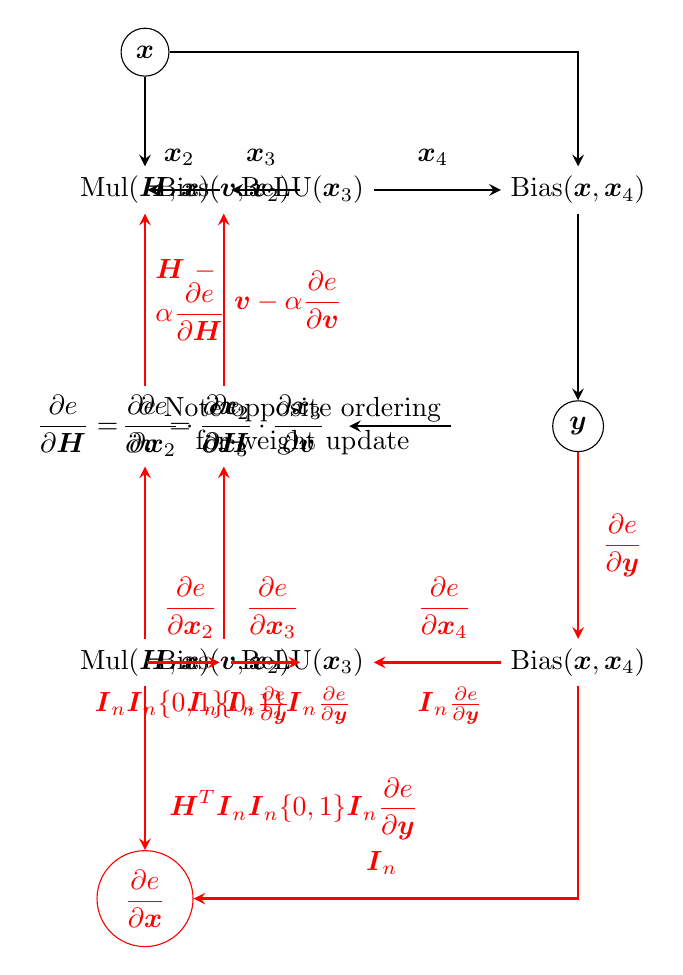
\begin{tikzpicture}[x=1.5cm, y=1.5cm, >=stealth]

		% Dense
		\node [every block/.try, block forw-1/.try] (forw-1) at (0,4) {
			Mul$(\bs{H}, \bs{x})$
		};
		\node [block backward/.try, block forw-1/.try] (back-1) at (0,0) {
			Mul$(\bs{H}, \bs{x})$
		};
		\node [block backward/.try, block forw-1/.try] (h-1) at (0,2) {
			$\dfrac{\pd e}{\pd \bs{H}}=
			\dfrac{\pd e}{\pd \bs{x}_2}\cdot\dfrac{\pd \bs{x}_2}{\pd\bs{H}}$
		};

		% Bias
		\node [every block/.try, block forw-2/.try, right of=forw-1] (forw-2) {
			Bias$(\bs{v}, \bs{x}_2)$
		};
		\node [block backward/.try, block back-2/.try, right of=back-1] (back-2) {
			Bias$(\bs{v}, \bs{x}_2)$
		};
		\node [block backward/.try, block forw-2/.try, right of=h-1] (h-2) {
			$\dfrac{\pd e}{\pd \bs{v}}=
			\dfrac{\pd e}{\pd \bs{x}_3}\cdot\dfrac{\pd \bs{x}_3}{\pd\bs{v}}$
		};

		% RELU
		\node [every block/.try, block forw-3/.try, right of=forw-2] (forw-3)  {
			ReLU$(\bs{x}_3)$
		};
		\node [block backward/.try, block back-3/.try, right of=back-2] (back-3)  {
			ReLU$(\bs{x}_3)$
		};
		\node [block backward/.try, block forw-2/.try, right of=h-2, draw=none,
			color=black, align=center] (h-3) {
			Note opposite ordering \\
			for weight update
		};

		% Residual bias
		\node [every block/.try, block forw-4/.try, right of=forw-3, node
		distance=3.5cm] (forw-4)  {
			Bias$(\bs{x}, \bs{x}_4)$
		};
		\node [block backward/.try, block back-4/.try, right of=back-3, node
		distance=3.5cm] (back-4)  {
			Bias$(\bs{x}, \bs{x}_4)$
		};
		\node [block backward/.try, block forw-2/.try, right of=h-3, draw=none,
		node distance=3.5cm] (h-4) {
		};

		% x input
		\node [circle, draw, above of=forw-1, node distance=1.75cm] (xin) {$\bs{x}$};

		% y output
		\node [circle, draw, right of=h-4, node distance=0cm]
			(y) {$\bs{y}$};

		\draw [->, line width=0.3mm] (forw-4) -- (y);
		\draw [->, line width=0.3mm] (xin) -- (forw-1);
		\draw [->, line width=0.3mm] (xin) -| (forw-4);
		\draw [->, line width=0.3mm, color=red] (y) --
			node [text width=0.5cm,midway, right=0.5em] {
				$\dfrac{\pd e}{\pd \bs{y}}$
			}
			(back-4);
		\draw [->, line width=0.3mm, color=black, shorten >=0.5em] (h-3) -- (h-2);

		\foreach \l [count=\i] in {2, 3, 4}
			\draw [->, line width=0.3mm] (forw-\i) --
				node [text width=0.5cm,midway,above=0.5em] {$\bs{x}_\l$}
				(forw-\l);



		\draw [->, line width=0.3mm, color=red] (back-4) --
			node [text width=0.5cm,midway,below=0.5em] {
				$\bs{I}_n\frac{\pd e}{\pd\bs{y}}$
			}
			node [text width=0.5cm,midway,above=0.5em] {
				$\dfrac{\pd e}{\pd \bs{x}_4}$
			}
			(back-3);
		\draw [->, line width=0.3mm, color=red] (back-3) --
			node [text width=2cm,midway,below=0.5em] {
				$\bs{I}_n\{0, 1\}\bs{I}_n\frac{\pd e}{\pd\bs{y}}$
			}
			node [text width=0.5cm,midway,above=0.5em] {
				$\dfrac{\pd e}{\pd \bs{x}_3}$
			}
			(back-2);
		\draw [->, line width=0.3mm, color=red] (back-2) --
			node [midway, text width=2.25cm,midway,below=0.5em] {
				$\bs{I}_n\bs{I}_n\{0, 1\}\bs{I}_n\frac{\pd e}{\pd\bs{y}}$
			}
			node [text width=0.5cm,midway,above=0.5em] {
				$\dfrac{\pd e}{\pd \bs{x}_2}$
			}
			(back-1);

		\node [circle, draw, below of=back-1, node distance=3cm, color=red] (xback) {
			$\dfrac{\pd e}{\pd \bs{x}}$
		};
		\draw [->, line width=0.3mm, color=red] (back-1) --
			node [text width=0.5cm,near end,right=0.5em] {
				$\bs{H}^T\bs{I}_n\bs{I}_n\{0, 1\}\bs{I}_n\dfrac{\pd e}{\pd\bs{y}}$
			}
			(xback);
		\draw [->, line width=0.3mm, color=red] (back-4) |-
			node [text width=0.5cm,near end,above=0.5em] {
				$\bs{I}_n$
			}
		(xback);

		% Grad arrows
		\foreach \l in {1, 2}
			\draw [->, line width=0.3mm, color=red] (back-\l) --
				(h-\l);
		\draw [->, line width=0.3mm, color=red] (h-1) --
			node [text width=1.5cm,midway,right=0em] {
				$\bs{H} - \alpha\dfrac{\pd e}{\pd \bs{H}}$
			}
			(forw-1);
		\draw [->, line width=0.3mm, color=red] (h-2) --
			node [text width=1.5cm,midway,right=0em] {
				$\bs{v} - \alpha\dfrac{\pd e}{\pd \bs{v}}$
			}
			(forw-2);

	\end{tikzpicture}
	\caption{Chain rule applied over backwards pass}
	\end{figure}

\end{proof}


% ---------------------------------------------------------
\HomeworkHeader{3 (Calculus)}{6}% homework number, problem number
% ---------------------------------------------------------

\begin{solution}
	At the end of the last problem we created a graph depicting the backward
	pass and how gradients flow across blocks. This graph also shows the
	generic form of the gradient descent updates. All we have to do is express
	these generic forms in terms of known variables

	\begin{align}
		\bs{H} - \alpha \frac{\pd e}{\pd \bs{H}}
		&= \bs{H} - \alpha \bigg(
			\frac{\pd e}{\pd \bs{x}_2}\cdot\frac{\pd\bs{x}_2}{\pd\bs{x}}
		\bigg)
		\\
		&= \bs{H} - \alpha \Bigg(
			\bigg(
				\bs{I}_n\bs{I}_n\{0, 1\}\bs{I}_n\dfrac{\pd e}{\pd\bs{y}}
			\bigg)
			\cdot
			\bigg(
				\bs{x}^T
			\bigg)
		\Bigg)
	\end{align}
	\begin{align}
		\bs{v} - \alpha \frac{\pd e}{\pd \bs{v}}
		&= \bs{v} - \alpha \bigg(
			\frac{\pd e}{\pd \bs{x}_3}\cdot\frac{\pd\bs{x}_3}{\pd\bs{x}_2}
		\bigg)
		\\
		&= \bs{v} - \alpha \Bigg(
			\bigg(
				\bs{I}_n\{0, 1\}\bs{I}_n\dfrac{\pd e}{\pd\bs{y}}
			\bigg)
			\cdot
			\bigg(
				\bs{I}_n
			\bigg)
		\Bigg)
	\end{align}

	For the multiplication block we see that the weight update depends in part on
	$\bs{x}$. As such, we will need to store $\bs{x}$ from the forward pass in
	order to perform gradient descent during the backward pass.

	Furthermore, the diagonal matrix produced as we differentiate ReLU will
	depend on what inputs were given to ReLU in the forward pass. Thus we must
	store input $\bs{x}_3$ where we map $x_i \in \bs{x}_3 < 0$ to $0$ in
	$\bs{I}\{0, 1\}$.

\end{solution}

% ---------------------------------------------------------
\HomeworkHeader{3 (Calculus)}{7}% homework number, problem number
% ---------------------------------------------------------

\begin{solution}
	This problem expands on the summation proved in the last homework. Slide 76
	of the linear algebra lecture provides a nice picture of what is going on.
	The yellow dense Toeplitz matrix for $\bs{X}$ shows concretely the role of
	edge effects in producing varying numbers of duplicated filter weights.
	Such edge effects are the result of elements in an input feature map being
	passed over by a varying number of filter kernel weights based on their
	location. For example, column edge elements will receive only one filter
	weight across a given row, while inner elements will be exposed to the
	filter kernel multiple times.

	In order to avoid wasting memory on duplicated inputs we do not store the
	entire Toeplitz matrix. From the picture on slide 76 it is clear that
	no duplications occur along a row of the Toeplitz matrix. It is also clear
	from the indexing for $\bs{X}_{f_rf_c}$ given in the problem that a row of
	the Toeplitz matrix contains inputs of one feature map that are all passed
	over by the same filter coefficient. As such, skipping $F_r * F_c$ rows
	will take us between input feature maps.
	\newline

	With that background, we can start by drawing a rough approximation of the
	summation of matrix matrix multiplications as follows.



	\tikzset{%
		every block/.style={
			rectangle,
			draw,
			minimum width=3cm,
			minimum height=1cm,
			node distance=2cm
		},
		every input/.style={
			circle,
			draw,
			minimum size=1.25cm,
			node distance=2cm
		},
		backward/.style={
			color=red
		},
		phantom node/.style={
			rectangle,
			draw=none,
			minimum width=1cm,
			minimum height=1cm,
			node distance=2cm
		},
		missing/.style={
			draw=none,
			scale=4,
			text height=0.333cm,
			execute at begin node=\color{black}$\vdots$
		},
	}

	\begin{figure}[H]
	\centering
	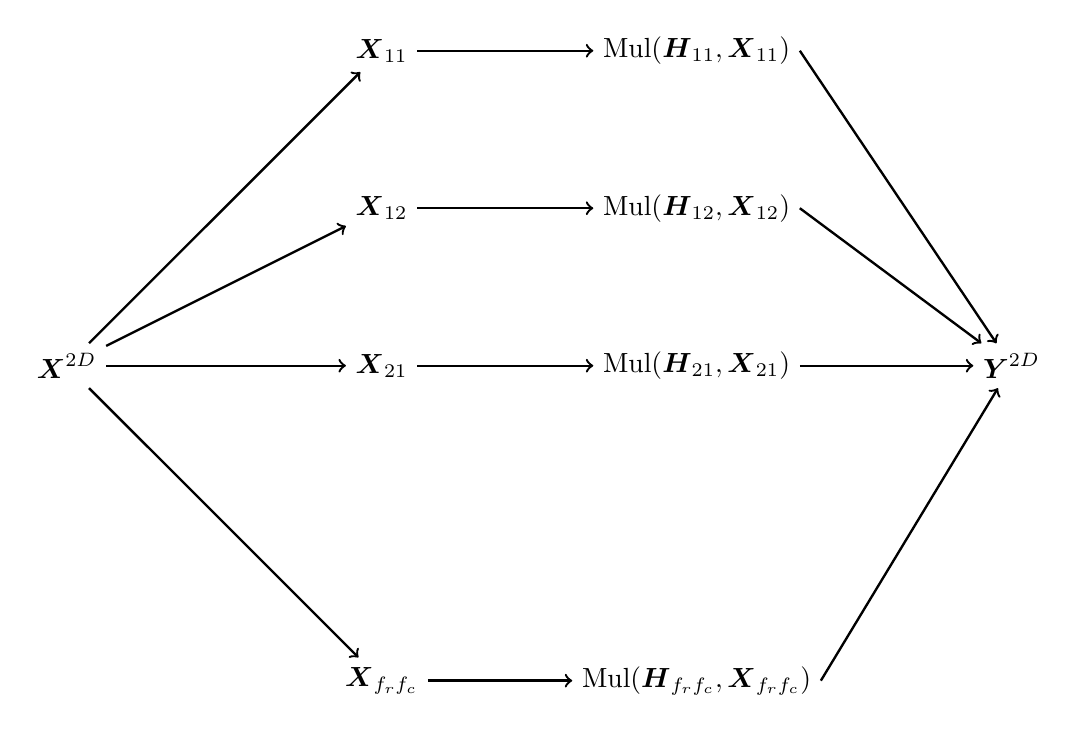
\begin{tikzpicture}
		\foreach \l [count=\i] in {11,12,21,missing,f_rf_c} {
			\node [every input/.try, \l/.try] (x-\l) at (0,{-2*\i}) {
				\ifstringequal{\l}{missing}{}{$\bs{X}_{\l}$}
			};
			\node [every block/.try, \l/.try] (h-\l) at (4,{-2*\i}) {
				\ifstringequal{\l}{missing}{}
				{Mul$(\bs{H}_{\l}, \bs{X}_{\l})$}
			};
			\ifstringequal{\l}{missing}
				{}
				{
					\draw [->, line width=0.3mm] (x-\l) -- (h-\l)
			};
		};

		\node [every input/.try] (y) at (8,-6) {
			$\bs{Y}^{2D}$
		};
		\foreach \l [count=\i] in {11,12,21,f_rf_c} {
			\draw [->, line width=0.3mm, color=black] (h-\l.east) --
			(y);
		};

		\node [every input/.try] (x) at (-4,-6) {
			$\bs{X}^{2D}$
		};
		\foreach \l [count=\i] in {11,12,21,f_rf_c} {
			\draw [->, line width=0.3mm, color=black] (x) --
			(x-\l);
		};
	\end{tikzpicture}
	\caption{Outline of CNN style 2D convolution as sum of matrix
		multiplications}
	\end{figure}

	\begin{figure}[H]
	\centering
	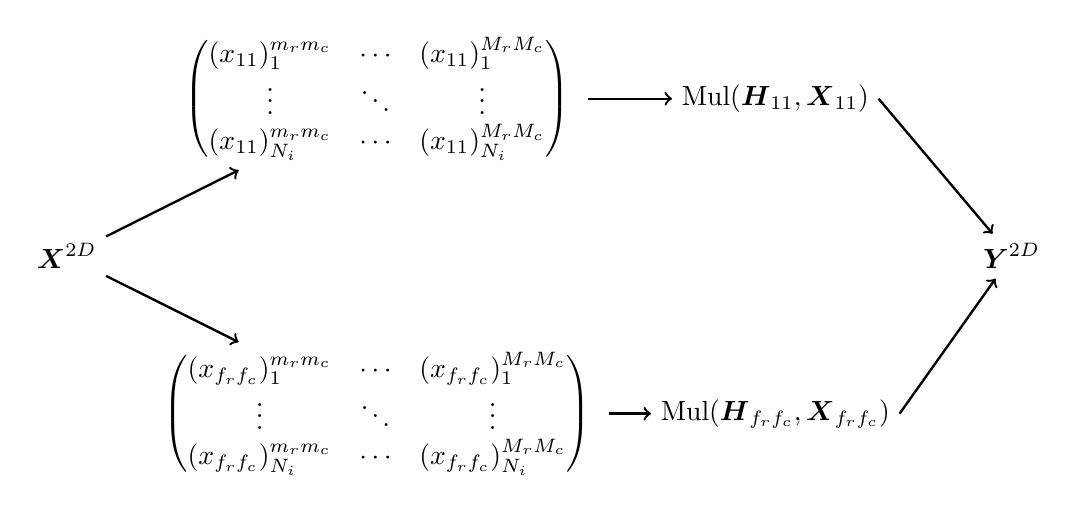
\begin{tikzpicture}
		\node [every input/.try] (x) at (-4,-4) {
			$\bs{X}^{2D}$
		};
		\node [every input/.try] (y) at (8,-4) {
			$\bs{Y}^{2D}$
		};
		\foreach \l [count=\i] in {11,missing,f_rf_c} {
			\node [every block/.try, \l/.try] (x-\l) at (0,{-2*\i}) {
				\ifstringequal{\l}{missing}{}{
					$\begin{pmatrix}
						(x_{\l})_{1}^{m_rm_c} & \cdots & (x_{\l})_{1}^{M_rM_c}\\
						\vdots & \ddots & \vdots \\
						(x_{\l})_{N_i}^{m_rm_c} & \cdots & (x_{\l})_{N_i}^{M_rM_c}\\
					\end{pmatrix}$
				}
			};
			\node [every block/.try, \l/.try] (h-\l) at (5,{-2*\i}) {
				\ifstringequal{\l}{missing}{}
				{Mul$(\bs{H}_{\l}, \bs{X}_{\l})$}
			};
			\ifstringequal{\l}{missing}
				{}
				{
					\draw [->, line width=0.3mm] (x-\l) -- (h-\l.west);
					\draw [->, line width=0.3mm, color=black] (h-\l.east) --
					(y);
					\draw [->, line width=0.3mm, color=black] (x) --
					(x-\l);
			};
		};

	\end{tikzpicture}
	\caption{Attempt at showing matrices that contribute to the summation}
	\end{figure}

	We can then draw a \textbf{rough} outline of the backward pass

	\begin{figure}[H]
	\centering
	\begin{tikzpicture}
		\foreach \l [count=\i] in {11,12,21,missing,f_rf_c} {
			\node [every input, backward, \l/.try] (x-\l) at (0,{-2*\i}) {
				\ifstringequal{\l}{missing}{}{
					$\dfrac{\pd e}{\pd\bs{X}_{\l}}$
				}
			};
			\node [every block, backward, \l/.try] (h-\l) at (4,{-2*\i}) {
				\ifstringequal{\l}{missing}{}
				{
					$\hat{\bs{H}}_{\l}^T$
				}
			};
			\ifstringequal{\l}{missing}
				{}
				{
					\draw [<-, backward, line width=0.3mm] (x-\l) -- (h-\l)
			};
		};

		\node [every input, backward] (y) at (8,-6) {
			$\dfrac{\pd e}{\pd\bs{Y}}$
		};
		\foreach \l [count=\i] in {11,12,21,f_rf_c} {
			\draw [<-, backward, line width=0.3mm] (h-\l.east) --
			(y);
		};

		\node [every input, backward] (x) at (-4,-6) {
			$\dfrac{\pd e}{\pd\bs{X}}$
		};
		\foreach \l [count=\i] in {11,12,21,f_rf_c} {
			\draw [<-, backward, line width=0.3mm] (x) --
			(x-\l);
		};
	\end{tikzpicture}
	\caption{Backward pass outline of CNN style 2D convolution as sum of matrix
		multiplications}
	\end{figure}

	First, note that the backward pass strongly resembles a
	forward pass, but acting on differently shaped input with transposed
	block diagonal filters. As such, we should be able to express
	the backward pass as a CNN
	style 2D convolution or equivalent sum of lowered matrix matrix
	multiplications. However, to express the backpropagation step as a lowered
	CNN style 2D convolution we would need to modify $\pd e / \pd\bs{Y}$ in the
	same way we did $\bs{X}$ in the original lowering.
	\newline

	This would let us write something like

	\begin{align}
		\frac{\pd e}{\pd\bs{X}^{2D}}
		&=
		\sum_{f_rf_c}\bigg(\bs{H}_{f_rf_c}^{2D}\bigg)^T
		\frac{\pd e}{\pd \bs{Y}_{f_rf_c}^{2D}}
	\end{align}

	with associated CNN style 2D convolution

	\begin{align}
		\frac{\pd e}{\pd\bs{X}}
		&=
		\bs{H}^T
		\frac{\pd e}{\pd \bs{Y}}
	\end{align}

	My best guess on how to create $\bs{Y}^{2D}$ is that we would
	follow the process by which the Toeplitz matrix created $\bs{X}^{2D}$.
	We could express $(\bs{H}^{2D})^T$ as $N_i \times (N_o F_r F_c)$ and
	$\bs{Y}^{2D}$ as $N_o F_r F_c \times M_r M_c$. If we then pad $\bs{Y}^{2D}$
	appropriately such that we convert $M_r, M_c$ to $L_r L_c$ we would have a
	lowered matrix matrix expression that would produce the correct output. The
	padding would be probably be more easily visualized if it was applied using
	normal convolution padding/stride rules before lowering $\bs{Y}$.



\end{solution}

% ---------------------------------------------------------
\HomeworkHeader{3 (Calculus)}{8}% homework number, problem number
% ---------------------------------------------------------
\begin{solution}
	Complete

	I tried doubling various parameters and for the most part the impact on
	training  time and accuracy was negligible. However, doubling the number of
	output feature maps or adding additional layers did create a substantial
	impact. It was a nice reflection that network design is not arbitrary, and
	that guessing network architecture would involve a lot of trial and error.
\end{solution}
% ---------------------------------------------------------
\HomeworkHeader{3 (Calculus)}{9}% homework number, problem number
% ---------------------------------------------------------
\begin{solution}Complete\end{solution}

\end{document}
